\documentclass[UTF8, fontset=windows]{article}
\usepackage[
    left=1.2in,
    right=1.2in,
    top=0.4in,
    bottom=0.7in,
    paperheight=11in,
    paperwidth=8.5in
]{geometry}
\usepackage[UTF8, nocap]{ctex}

\usepackage{layout}
\usepackage{amsmath}
\usepackage{algorithm}
\usepackage{algorithmic}
\usepackage{graphicx}
\usepackage{hyperref}
\usepackage{float}

\title{A multi-objective approach for energy-efficient and reliable dynamic VM
consolidation in cloud data centers \large \\Paper Summary}

\author{Summarized by: 武泽恺\\
  \small Student ID: 10225101429\\
}
\date{\vspace{-5ex}}

\begin{document}
\maketitle

\noindent Paper Link \cite{sayadnavard2022multi}: {\url{https://www.sciencedirect.com/science/article/pii/S221509862100104X}}

\section{Background}

The rapid growth of cloud computing has led to a huge amount of energy consumption in cloud data centers, since the inefficient use of the resources results in high operating costs and carbon emissions. Dynamic virtual machine (VM) consolidation is a strategy to address this issue by executing VMs on as few physical machines (PMs) as possible, reducing the number of PMs powered on and hence the energy consumption. However, this process should carefully optimize resource utilization while meeting Service Level Agreements (SLAs) and Quality of Service (QoS) requirements, which is not achieved in the existing literature \cite{beloglazov2012managing,li2017bayesian,zhang2015burstiness,mahdhi2018prediction,ponraj2019optimistic,shen2018compvm,speitkamp2010mathematical}.

\section{Problem Statement}

The paper addresses the challenge of achieving energy-efficient and reliable dynamic VM consolidation in cloud data centers. The primary issues are the degradation of system performance and reliability, as well as the violation of SLAs and QoS requirements due to the high frequency of VM consolidation and the placement of VMs on unreliable PMs.

From my perspective, this problem is not only realistic but also crucial. Nowadays, with the development of the digital economy, cloud services play an increasingly significant role in various industries. This problem directly impacts the cost and reliability of cloud services. Therefore, finding an effective solution is essential for cloud service providers to maintain high reliability and sustainability.

\section{Methodology}

The discussed system architecture is shown in Figure \ref{fig:architecture}, which consists of two kinds of agents: fully distributed local agents in each PM, and a global agent in a master node. 

\begin{figure}[h]
  \centering
  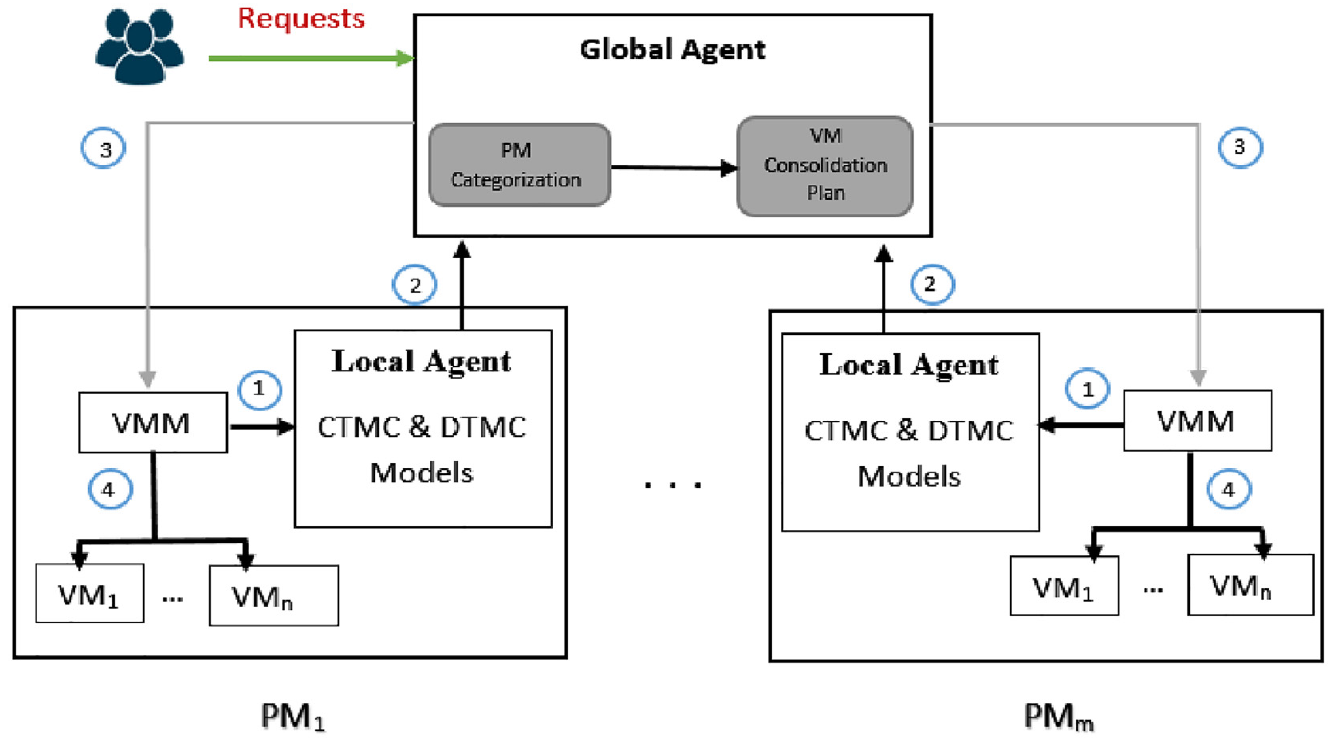
\includegraphics[width=0.8\textwidth]{images/architecture.png}
  \caption{System architecture.}
  \label{fig:architecture}
\end{figure}

In the proposed method, the local agents are responsible for monitoring the PM status and reliability, predicting the future status and reliability using Discrete-Time Markov Chain (DTMC) and Continuous Time Markov Chain (CTMC), respectively. The global agent uses the predicted PM status and reliability to optimize the VM consolidation process using an enhanced Multi-Objective Artificial Bee Colony ($\epsilon$-MOABC) algorithm. The main steps are presented in Figure \ref{fig:method}.

\begin{figure}[h]
  \centering
  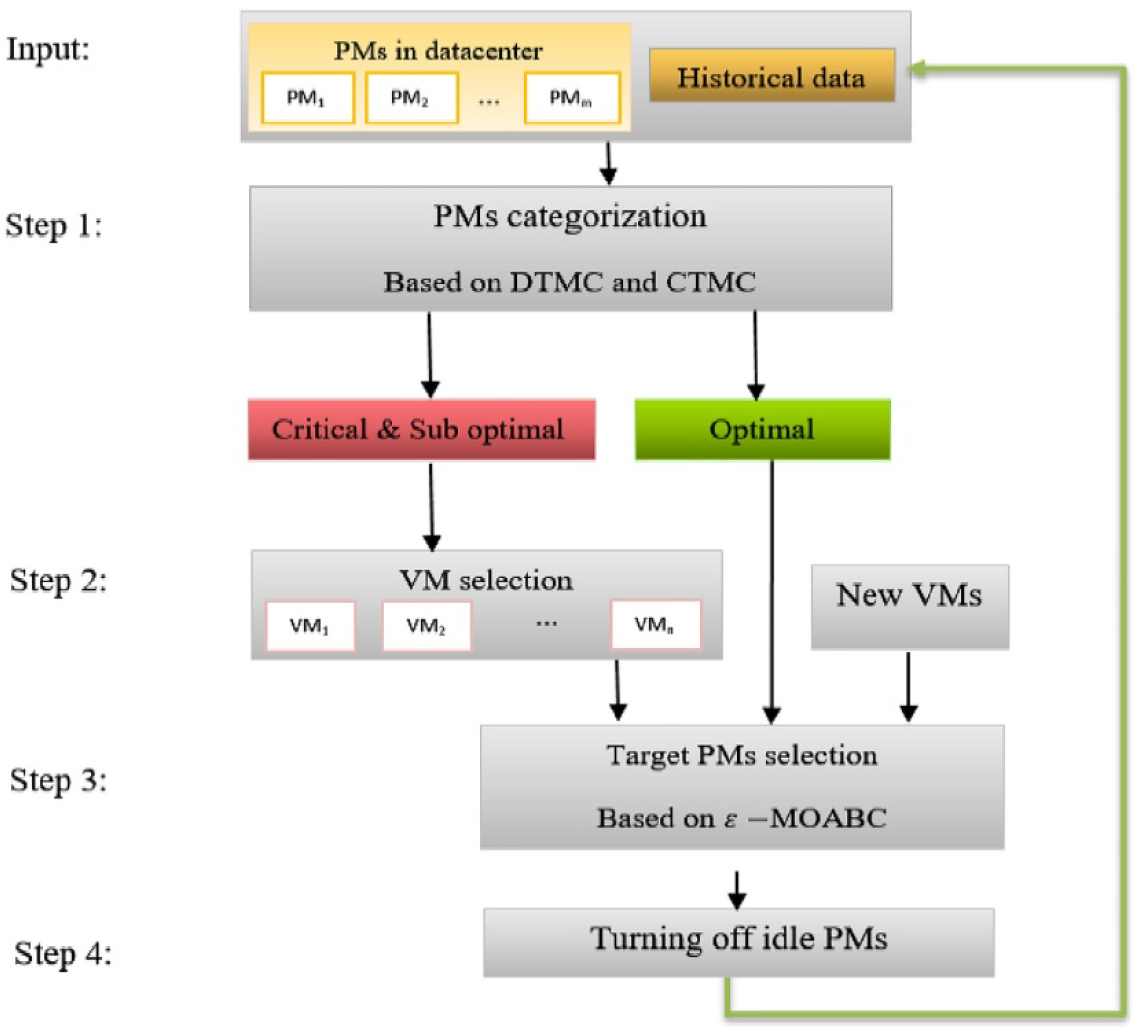
\includegraphics[width=0.6\textwidth]{images/method.png}
  \caption{Proposed VM consolidation approach.}
  \label{fig:method}
\end{figure}

First, based on historical data like CPU utilization, memory usage, and storage, the local agent predicts the future PM status using the DTMC model, which constructs the matrix of transition probabilities between different states. The CTMC model is then used to predict the future reliability of PMs, which considers the time to transit from one system state to another due to failures and recovery using an exponential distribution. The state transition diagram for DTMC and CTMC is shown in Figure \ref{fig:dtmc}.

\begin{figure}[h]  
  \centering
  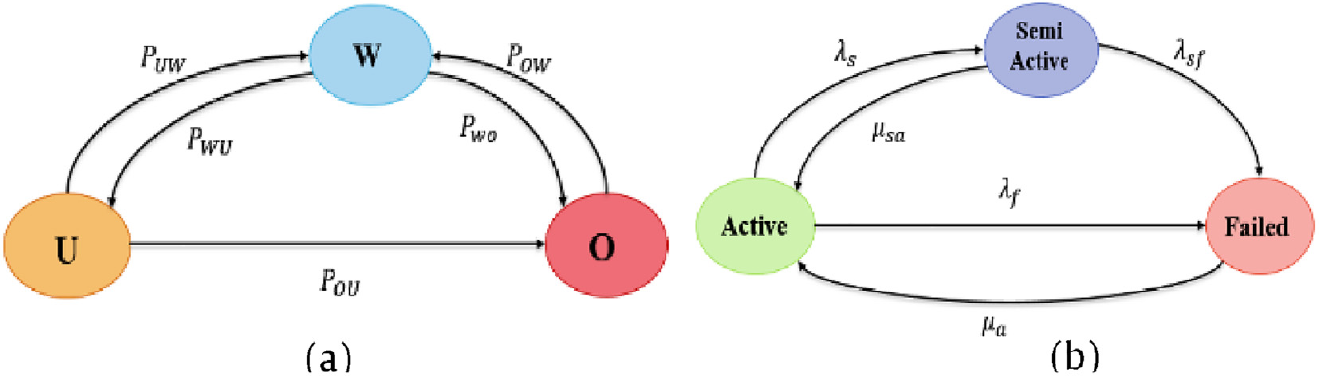
\includegraphics[width=0.8\textwidth]{images/transition.png}
  \caption{State transition diagram (a) DTMC (b) CTMC.}
  \label{fig:dtmc}
\end{figure}

Afterward, as presented in Algorithm \ref{alg:categorization}, the global agent gathers the predicted data and categorizes PM status into three states: Under-loaded, Overloaded, and Well-utilized, and also classifies reliability as Reliable or Unreliable, resulting in six possible states (WR, UR, OR, UU, OU, WU).

Then, the authors introduce a heuristic VM selection algorithm, shown in Algorithm \ref{alg:vm_selection}, that considers both the estimated finishing time (EFT) of a virtual machine for all the assigned tasks and migration time. If the EFT is less than the mean first passage time (MFPT) of the current PM, the VM will not be selected for migration. Otherwise, the algorithm calculates a score for each dissatisfied VM based on host load changes and memory usage and selects the VM with the lowest score for migration. The score is calculated using Equation \ref{eq:score}.

\begin{equation}
  \text{Score}_i = \omega \cdot \frac{\frac{\text{Mem}_i}{\text{BW}_j} - \left(\frac{\text{Mem}}{\text{BW}}\right)_{\text{min}}}{\left(\frac{\text{Mem}}{\text{BW}}\right)_{\text{max}} - \left(\frac{\text{Mem}}{\text{BW}}\right)_{\text{min}}} 
  + (1 - \omega) \cdot \frac{\Delta U^{\text{cpu}}_{\text{max}} - \Delta U^{\text{cpu}}_i}{\Delta U^{\text{cpu}}_{\text{max}} - \Delta U^{\text{cpu}}_{\text{min}}}
\label{eq:score}
\end{equation}

Finally, the $\epsilon$-MOABC algorithm is adopted to optimize the VM consolidation process, which is an improved version of the multi-objective artificial bee colony (MOABC) algorithm. The algorithm is designed to minimize energy consumption, and resource wastage, and maximize system reliability. The pseudocode is presented in Algorithm \ref{alg:moabc}.

Based on the MOABC algorithm, the $\epsilon$-MOABC algorithm first initializes a population of solutions. Then, it assigns \texttt{employed bees} to explore and improve these solutions using differential evolution. Afterward, the best findings are shared with \texttt{onlooker bees} to calculate the fitness value of the solutions. Besides, \texttt{scout bees} are sent to find abandoned solutions that can not be optimized and reset them. At the end of each iteration, the non-dominated solutions are stored in an archive with a limited size. The algorithm iterates until the maximum number of iterations is reached, and the best solution with
the highest binary indicator value is selected from the archive.

\section{Innovation}

The paper primarily introduces three innovative insights, including:

\begin{itemize}
  \item Combining DTMC and CTMC for PM categorization to predict future resource usage and system behavior.
  \item Introducing a heuristic approach that reduces unnecessary migrations by considering migration time and task completion time.
  \item Using $\epsilon$-MOABC to address conflicting objectives such as energy reduction and reliability maximization.
\end{itemize}

In my opinion, this paper has carefully considered energy efficiency, resource optimization, and system reliability simultaneously, which are overlooked in the previous works. Also, the technical depth is substantial since it involves reasonable models and optimization algorithms to address this complex problem.

\section{Strengths}

The paper has several strengths, including:

\begin{itemize}
  \item The paper addresses multiple objectives (energy consumption, resource wastage, system reliability) simultaneously, which provides a comprehensive solution to the VM consolidation problem that can be applied in practice.
  \item This paper incorporates PM reliability into decision-making, preventing additional migrations and system failures. As we discussed, this is a crucial aspect often overlooked in existing literature.
  \item The use of the $\epsilon$-MOABC algorithm for multi-objective optimization is a creative solution that balances competing factors effectively. It combines the biological behavior of bees with the optimization process, which is a great innovation.
  \item Extensive experimental results are provided to validate the proposed approach, where many existing methods like LR-MMT, LR-MC, LR-RS, MAD-MMT, MAD-MC, MAD-RS, IQR-MMT, IQR-MC, and IQR-RS are compared, improving the credibility of the solution (See Section 5.4 in the original paper).
\end{itemize}

\section{Deficiencies}

Despite the strengths, the paper also has some limitations, including:

\begin{itemize}
  \item As far as I know, latency is also a critical factor in cloud environments, a QoS parameter that is not directly optimized in this method. It would be beneficial to consider latency in the optimization process.
  \item As the authors mentioned, the complexity of the implementation on a real cloud platform could be a challenge. Therefore, they use the CloudSim toolkit for simulation. From my perspective, a real-world deployment would be more convincing, if possible.
\end{itemize}

\begin{figure}[b]
  \centering
  \begin{minipage}[t]{0.45\textwidth}
      \begin{algorithm}[H]
          \caption{Categorization}
          \begin{algorithmic}[1]
          \REQUIRE PMs status
          \ENSURE Categories
          \FOR{each host in PM set}
              \IF{PM\_state = OU $|$ OR $|$ WU}
                  \STATE Add to Critical\_cat
              \ELSIF{PM\_state = WR}
                  \STATE Add to Optimal\_cat
              \ELSIF{PM\_state = UR $|$ UU}
                  \STATE Add to SubOptimal\_cat
              \ENDIF
          \ENDFOR
          \RETURN Categories
          \end{algorithmic}
          \label{alg:categorization}
      \end{algorithm}
  \end{minipage}
  \hfill
  \begin{minipage}[t]{0.45\textwidth}
      \begin{algorithm}[H]
          \caption{VM selection}
          \begin{algorithmic}[1]
          \REQUIRE $PM_i$ ($PMs$ in $OR\_list$, $OU\_list$, $WU\_list$) // Source PMs
          \ENSURE VM migration list
          \STATE $Migration\_list = 0$
          \FOR{each PM in $PMlist$}
              \STATE $VM\_list = PM.getVmList()$
              \IF{current\_state = WR}
                  \FOR{each $VM_i$ in $VM\_list(PM_j)$}
                      \IF{$ECT_{VM} < MFPT_{PM}$}
                          \STATE $VM\_list(PM_i) = VM\_list(PM_j) - \{VM_i\}$
                      \ENDIF
                  \ENDFOR
              \ENDIF
              \WHILE{$VM\_list(PM_j) = true$ \AND $PM_j\_load > High\_Tr$}
                  \FOR{each $VM_i$ in $VMlist(PM_j)$}
                      \STATE Calculate $Score_i$ using Eq.~(11)
                      \IF{$Score_i < Min\_Score$}
                          \STATE $Min\_Score = Score_i$
                          \STATE $Best\_VM = VM_j$
                      \ENDIF
                  \ENDFOR
                  \STATE Insert $Best\_VM$ in $Selected\_VM$ list
                  \STATE $VMlist(PM_j) = VMlist - \{Selected\_VM\}$
                  \STATE Calculate new $PM_j\_load$
              \ENDWHILE
              \STATE $Migration\_list = Migration\_list \cup \{Selected\_VM\}$
          \ENDFOR
          \RETURN $Migration\_list$
          \end{algorithmic}
          \label{alg:vm_selection}
      \end{algorithm}
  \end{minipage}
\end{figure}

\begin{algorithm}[b]
  \caption{$\varepsilon$-MOABC based VM placement}
  \begin{algorithmic}[1]
  \REQUIRE Migration\_list, WR\_list, UR\_list
  \ENSURE Migration plan (Mapping of each VMs to PMs)
  \STATE Set the parameter Population size, Archive size, trial\_limit, $iter_{max}$
  \STATE Randomly initialize a population $X = (x_1, x_2, \ldots, x_N)$
  \STATE Evaluate fitness functions $f_1$, $f_2$ and $f_3$ for any individual $x_i$
  \STATE Start the optimization process:
  \WHILE{(iter $\leq iter_{max}$)}
      \FOR{$i = 1$ to FoodNumber // Employed Bees}
          \STATE Select one dimension $d$ and 3 neighbors $p$, $k$, and $q$ randomly
          \STATE Calculate new solution $v_i$ using Eq.~(27)
          \STATE Evaluate fitness functions for new solution (obtaining new solution)
          \STATE Calculate fitness based on indicator $I_{\varepsilon}$ using Eq.~(28) and Eq.~(29)
          \IF{$I(v_i) > I(x_i)$}
              \STATE Add $v_i$ to the archive
              \STATE $x_i = v_i$
              \STATE $trial_i = 0$
          \ELSE
              \STATE $trial_i = trial_i + 1$
          \ENDIF
      \ENDFOR
      \STATE Calculate the probabilities of each solution using Eq.~(30) // Onlooker Bees
      \STATE $i = 0$, $t = 0$
      \WHILE{$t < \text{FoodNumber}$}
          \IF{$rand < P_i$}
              \STATE $t = t + 1$
              \STATE Select one dimension $d$ and 3 neighbors $p$, $k$, and $q$ randomly
              \STATE Evaluate fitness functions for new solution
              \STATE Calculate fitness based on indicator $I_{\varepsilon}$ using Eq.~(28) and Eq.~(29)
              \IF{$I(v_i) > I(x_i)$}
                  \STATE Add $v_i$ to the archive
                  \STATE $x_i = v_i$
                  \STATE $trial_i = 0$
              \ELSE
                  \STATE $trial_i = trial_i + 1$
              \ENDIF
          \ENDIF
          \STATE $i = i + 1$
          \IF{$i == \text{FoodNumber}$}
              \STATE $i = 1$
          \ENDIF
      \ENDWHILE
      \FOR{$i = 1$ to FoodNumber // Scout Bees}
          \IF{$\max(trial_i) > trial\_limit$}
              \FOR{$d = 1$ to $D$}
                  \STATE $x_{id} = \text{round}(l_b + \text{rand}(0.1) * (u_b - l_b))$
              \ENDFOR
              \STATE $trial_i = 0$
          \ENDIF
      \ENDFOR
      \STATE Update Archive()
  \ENDWHILE
  \STATE Select the best solution from archive
  \RETURN Migration plan
  \end{algorithmic}
  \label{alg:moabc}
  \end{algorithm}

\bibliographystyle{ieeetr}
\bibliography{add}

\end{document}